\documentclass{article}
\usepackage{mathtools}
\usepackage[top=2in, bottom=1.5in, left=1in, right=1in]{geometry}
\usepackage{graphicx}
\usepackage[normalem]{ulem}
\usepackage{fancyhdr}
\pagestyle{fancyplain}
\usepackage{enumerate}
\usepackage{verbatim}

\rhead{A. Shawn Bandy 
(003635396)}
\lhead{Economics 485}
\begin{document}
\title{Homework \#4}
\author{A. Shawn Bandy}
\date{March 7th, 2013}
\maketitle

	\section{Lab Problems}
		\begin{enumerate}[L1]
			\item 
				\begin{description}
					\item{STATA code:}
						{\small {
							\verbatiminput{lab4.do}
						}}
					\item{Log output:}
						{\small {
							\verbatiminput{arclab.log}
						}}
					\item{Answers:}
						\begin{description}
							\item{f. What is the estimated slope coefficient for percoll90?  What is the interpretation of this slope coefficient?} \\
							
							The estimated slope is .0113436.  For each unit change in percoll90, there is a 0.113436 unit change in employment growth between 1990 and 2006.  It should be noted that in this  regression the value for percoll90 is not within the 95\% confidence interval and so there may be no realistic interpretation for the coefficient.\\
							
							\item{h. What is the estimated slope coefficient for percoll90 in the model from part g? What is the interpretation of this slope coefficient?}\\
							
							The estimate slope is .0180694.  For each unit change in percoll90, there is a .0180694 unit change in employment growth between 1990 and 2006, holding perse90 constant.  In this case the coefficient is in the 95\% confidence interval although it has very little impact on the dependent variable.\\
							
							\item{i. Using your results from parts e and g, does the regression model in part e suffer from omitted variable bias? Explain.}\\
							
							The model in part e suffers from omitted bias only if the additional variable, perse90, has a zero coefficient in the model in part g \emph{and} the omitted variable is correlated with percoll90.  The coefficient for perse90 in model g is \emph{not} zero within the 95\% confidence interval and there is a negative correlation between the variables.  We can conclude that there is omitted variable bias in model e.
							
						\end{description}
				\end{description}
			\item 
				\begin{description}
					\item{STATA code:}
						{\small {
							\verbatiminput{lab42.do}
						}}
					\item{Log output:}
						{\small {
							\verbatiminput{arclab2.log}
						}}
					\item{Answers:}
						\begin{description}
						
						\item{b. Does the STATA output from part a) include both the new variables? Explain what happened.}\\
						
						STATA omits an independent variable when there is a dependency between it and one or more other variables.  Running  \emph{regress pci90\_thousands percoll90 perse90 pci90} shows that there is a dependency between pci90\_thousands and pci90.\\
						
						\item{d. What is the coefficient on arc? What is the interpretation of this coefficient in our model?}\\
						
						The coefficient for arc is  -.0441713, so for each unit change in the variable arc there is about a 4\% drop in employment growth between 1990 and 2006.  Because the t-stat is -0.54 and compounded by having a coefficient fairly close to zero, we should interpret this as almost certainly having no meaning in our model.\\
						
						\item{f. Why did we exclude Georgia from the model in part e? What is the interpretation of the coefficient on state1 (Alabama)?}\\
						
						We excluded Georgia because not doing so for at least one categorical dummy variable leads to perfect multicollinearity.  In other words, if we included all the dummy variables then the sum of all dummy variables for each observation.  In another sense, the Georgia variable becomes the basis by which all other dummy variables are measured.  \\
						
						\item{i. Are there any problems with multicollinearity in your model? Explain.}\\
						
						The VIF($\hat{\beta}_i$)  for all variables in the regression is less than 5 (or less than 10) so I would say that our model is reasonably free of multicollinearity.  As a rule-of-thumb, multicollinearity is not considered high when VIF($\hat{\beta}_i$) is less than 5 (or less than 10, depending on the particular thumb).  \\
						
						\item{j. Compare the final model in part g to the model in L1, part g in terms of how much they explain the variance in employment growth. Explain.}\\
						
						$R^2$ is the measure of how much variation in the dependent variable is explained by the regression model.  In the L2.g model, adjusted $R^2$ is 0.1456.  In the L1.g model, adjusted $R^2$ is 0.0787 which is about half of the L2.g model.  The F-stat for both would lead us to reject the null hypothesis for the model at the 95\% confidence level.  In the L2.g model, the t-stat is low enough for popsqmi\_60 and rural that we cannot reject the null hypothesis, but these variables are correlated with others in the model and so should be left in.  \\
						
						\end{description}
				\end{description}
			\end{enumerate}

	\section{Questions}

		\begin{enumerate}[Q1]
			\item
Suppose you are interested in whether there is a gender bias in setting wages.
				\begin{enumerate}[a.]
					\item 
	
You get data from the Current Population Survey. You then use STATA to estimate a regression function as follows:

\begin{center}
$wage_i = \beta_0 + \beta_1 Female_i + \beta_2 Nonwhite_i + \beta_3 Union Member_i + \beta_4 Education_i + \beta_5 Experience_i + u_i $
\end{center}
\begin{samepage}
Some of the Stata output is as follows:

\nopagebreak
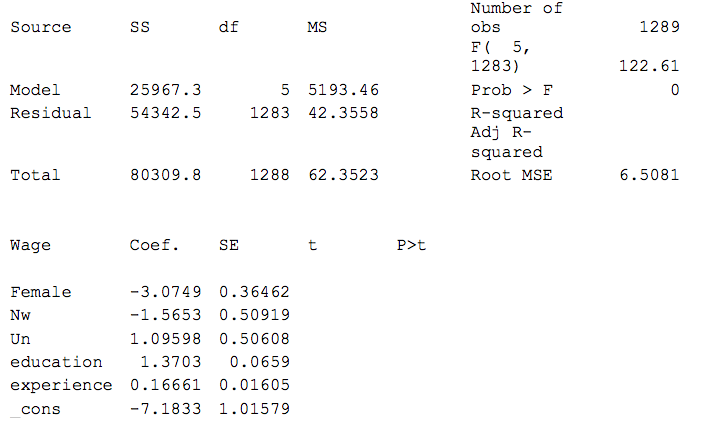
\includegraphics[width=400px]{q1_a_1}
\end{samepage}

What is the coefficient on female? What is the interpretation of this coefficient? Calculate the t-statistic and test whether it is statistically significant at the 5\% level. Based on the regression, do you think that women earn less than men?\\ 

The coefficient for female is -3.0749.  Holding all other variables in the model constant, being female reduces one's wages by -3.0749 dollars.\footnote{I am assuming the unit here is dollars.}  The t-statistic is calculated as $|\frac{\hat{\beta_1}}{SE}| = |\frac{-3.0749}{0.36462}| = |-8.43| >1.96$ so this variable is statistically significant at the 5\% level.  Yes, I would say based on this regression, women earn less than men.

				\item
What are the R2 and Adjusted R2 of this regression model?\\

$R^2$ equals 0.3233 and $\bar{R^2}$ equals 0.3207. 

 $R^2 \equiv 1 - \frac{SS_{residuals}}{SS_{total}} = 1 - \frac{54342.5}{80309.8} = 0.3233$
 
  $\bar{R^2} = 1 - \frac{SS_{residuals}}{SS_{total}}  * \frac{df_t}{df_e} = 1 - \frac{54342.5}{80309.8} * \frac{1288}{1283} = 0.3207$\\

				\item
As an alternative to the regression in part a, you collect data about gender and salaries from people who stop by a table at the local mall. You then use a �"difference in means" test to see if the average salary for women is less than the average salary for men. You find that there is a statistical difference in the means with women's average salary statistically lower than men's.\\

I see.\\

				\item
Even though both approaches give you the same answer, explain which method is a better way to test if women earn less than men.\\

Using the Current Population Survey is a much better method.  Sampling from a population is, at best, a means of estimating population parameters.  In this case, the sample size may be insufficient and the sample may in some way be self-selecting but more importantly a table at a local mall almost certainly does not adequately represent the population.  \\

				\item
\begin{samepage}
What if you also want to know whether women and men get the same additional wages for each additional year of school? To test this, you generate a new variable (female*education) which interacts the female dummy variable and education. The results of the regression are below:

\nopagebreak
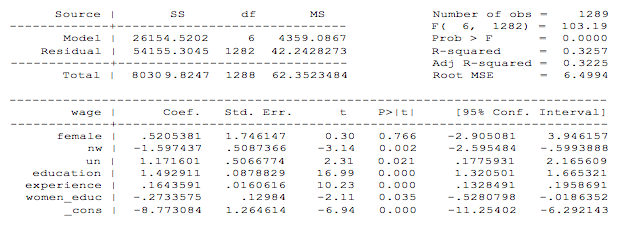
\includegraphics[width=400px]{q1_e_1}

What is the coefficient on women\_educ? Interpret the meaning of this coefficient in this regression model. \\

The coefficient on women\_educ is -0.2734 and it is statistically significant at the 5\% confidence level.  All other variables held constant, women receive -0.2734 fewer dollars per unit of education.  \footnote{I would have thought doing this would lead to a dependency issue if women\_educ is calculated directly from two other independent variables, but this does not appear to be an issue.}

\end{samepage}

				\end{enumerate}
		\item
Use the results from L1 to do the following. Follow the directions carefully in terms of what to calculate. Even if other parts of L1 include the answer, show how these elements are calculated, assuming you only had certain results. Please show the formula you use and the steps you take to get to the final answer. You can always use the output to see if you did it right!

			\begin{enumerate}[a.]
				\item
Use the results from L1 parts j and l to calculate the coefficient of percoll90 in the following regression model:

\begin{center}
$empgrowth\_9006_i = \beta_0 + \beta_1 percoll90_i + \beta_2 perse90_i + u_i$
\end{center}

I used the following formula to estimate $\beta_1$ : $\hat{\beta_1} = \frac{COV(empgrowth\_9006,residual)}{VAR(residual)} = \frac{.559228}{ 5.5682^2} = 0.01804$, where VAR(residual) = $Root MSE^2$\\
				\item

Calculate the t-statistic to test whether the coefficient on percoll90 is different than zero. Note: In this part it is OK to use the standard error calculated by the regression output rather than having to calculate it.\\

The t-statistic for $\hat{\beta_1}$ is 3.0157 which is greater than 1.96, making this statistically significant at the 95\% confidence interval and we can reject $H_0$.\\

I used  the following formula to estimate the t-stat value:  $t-stat = \frac{\hat{\beta_1}}{SE} = \frac{0.01804}{.0059809} = 3.0157$.\\
			\end{enumerate}
		\end{enumerate}
\end{document}